\section{DST}

 From the plot of the determinant of $S$ as a function of $n$ for $n$ from 1 to 32 shown in Figure~\ref{fig:S(n)}, it can be seen that the determinant has strictly discrete values of either 1 or -1 alternative every two values, and follows a sinusoidal pattern. It is also noticeable that the plot is an odd function.

    \begin{figure}[h!]
        \centering
        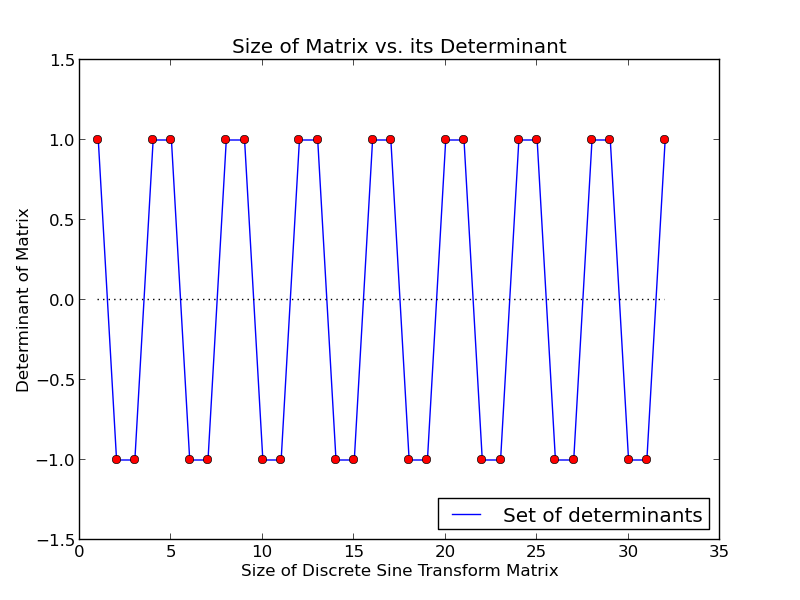
\includegraphics[scale=0.6]{./img/dst_dets.png}
        \caption{Determinants of $S(n)$}
        \label{fig:S(n)}
    \end{figure}

The equation used to create each of these matrices is expressed in \eqref{eq:dst}.

    \begin{equation}
        \label{eq:dst}
        S_{i,j}=\sqrt{\frac{2}{n}}sin \bigg(
        \frac{\pi(i-\frac{1}{2})(j-\frac{1}{2})}{n}\bigg)
    \end{equation}

The Python code used to generate the matrices as well as the graph is shown below.

    \lstinputlisting[language=Python,
                    showstringspaces=false,
                    frame=single,
                    firstline=194,
                    lastline=211,
                    basicstyle=\ttfamily,
                    keywordstyle=\color{blue},
                    numbers=left,
                    commentstyle=\color{red}]{./py/analysis.py}

    \lstinputlisting[language=Python,
                    showstringspaces=false,
                    frame=single,
                    firstline=229,
                    lastline=249,
                    basicstyle=\ttfamily,
                    keywordstyle=\color{blue},
                    numbers=left,
                    commentstyle=\color{red}]{./py/analysis.py}
